\subsection{Simple linear regression}

\begin{note}
  Consider the following simple example where we have:
  \begin{itemize}
    \item Rental price $p_r$ as our target feature, and
    \item Size $s$ as our descriptive (continuous) feature
  \end{itemize}
  We assume a linear dependency $p_r = b + a \cdot s$ and now want to base our prediction of the rental prize on the size. The example will guide us through this subchapter.
\end{note}

The \textbf{general problem}\sidenote{General problem regression} is given as follows:
\begin{itemize}
  \item We have given $n$ data rows in a set $\mathcal{D}$ with a target feature $t$ and descriptive features $\mathbf{d} = (d[1], d[2], \cdots, d[m])$, and
  \item We want to find a regression function $\mathbb{M}_\mathbf{w}$ with a constant weight and a weight for each feature, where
  \item We predict $\text{\color{mathblue}pred}(t) = \mathbb{M}_\mathbf{w}(\mathbf{d}) = \mathbb{M}_{(w[0], w[1], \cdots, w[m])}(d[1], d[2], \cdots, d[m])$
\end{itemize}
\begin{note}
  In our example, we only have one descriptive feature $\mathbf{d}=(d[1])$, two weights $\mathbf{w}=(w[0], w[1])$, and the regression function is linear, so $\underbrace{\mathbb{M}_\mathbf{w}(d)}_{p_r} = \underbrace{w[0]}_{b} + \underbrace{w[1]}_{a}\cdot\underbrace{d[1]}_{s}$. 
\end{note}

What can be seen is that the weights $\mathbf{w}=(w[0], w[1])$ define the linear function. Our goal is now to find the weights such that the resulting function has the "smallest error". There are different ways to characterize the error with different \textbf{error metrics}\sidenote{Error metrics}:
\begin{itemize}
  \item Sum of squared errors\sidenote{Sum of squared errors $L_2$} 
  \begin{align*}
    L_2(\mathbb{M}_\mathbf{w}, \mathcal{D}) = \frac{1}{2} \cdot \sum_{i=1}^n (t_i - \mathbb{M}_\mathbf{w}(d_i))^2
  \end{align*}
  \begin{note}
    \begin{itemize}
      \item For each instance: compute the error, then square it
      \item Compute the sum of the results
      \item Finally, take half ($\rightarrow$ end result)
    \end{itemize}
  \end{note}
  \item Mean squared error\sidenote{Mean squared error $MSE$} 
  \begin{align*}
    MSE(\mathbb{M}_\mathbf{w}, \mathcal{D}) = \frac{1}{n} \cdot \sum_{i=1}^n t_i - \mathbb{M}_\mathbf{w}(d_i)
  \end{align*}
  \item Root mean squared error\sidenote{Root mean squared error $RMSE$} 
  \begin{align*}
    RMSE(\mathbb{M}_\mathbf{w}, \mathcal{D}) = \sqrt{\frac{1}{n} \cdot \sum_{i=1}^n t_i - \mathbb{M}_\mathbf{w}(d_i)}
  \end{align*}
  \item Mean absolute error\sidenote{Mean absolute error $MAE$} 
  \begin{align*}
    MAE(\mathbb{M}_\mathbf{w}, \mathcal{D}) = \frac{1}{n} \cdot \sum_{i=1}^n \mid t_i - \mathbb{M}_\mathbf{w}(d_i) \mid
  \end{align*}
\end{itemize}

All of the introduced error metrics express the same idea, but usually, $L_2$ is chosen since it has a simple derivative. We'll take a look at the \textbf{partial derivative of error}, concretely of $L_2$ \begin{note}(here, $i$ refers to the training instance, and $j$ to one of the multiple descriptive features)\end{note}
\begin{align*}\begin{aligned}
  \frac{\delta}{\delta \mathbf{w}[j]}\ L_2(\mathbb{M}_\mathbf{w}, \mathcal{D}) 
    &= \frac{\delta}{\delta \mathbf{w}[j]}\ \frac{1}{2}\sum_{i=1}^n (t_i-\mathbb{M}_\mathbf{w}(d_i))^2\\
    &= - \sum_{i=1}^n \big((t_i - \mathbb{M}_\mathbf{w}(d_i)) \cdot d_i[j]\big)
\end{aligned}\end{align*}

Using this derivate, we can now find the weights minimizing the error. 
\begin{itemize}
  \item Brute force, meaning we try as many values as possible for the weights, isn't feasible in practice \begin{note}(not even for simple linear case)\end{note}.
  \item But we can use that our error surface is convex and therefore has a global minimum, enabling faster methods.
  \begin{itemize}
    \item Take the partial derivatives \begin{note}(for linear case: $\delta / \delta \mathbf{w}[0] \ L_2(\mathbb{M}_\mathbf{w}, \mathcal{D})$, and $\delta / \delta \mathbf{w}[1] \ L_2(\mathbb{M}_\mathbf{w}, \mathcal{D})$)\end{note}
    \item Find the correct values for all partial derivatives to result in zero \begin{note}(Needs to be the case for an actual global minimum)\end{note}
  \end{itemize}
\end{itemize}

One important thing to mention, the convex property of a function is very useful here:
\begin{figure}[H]
  \centering
  \begin{subfigure}{0.45\textwidth}
    \centering
    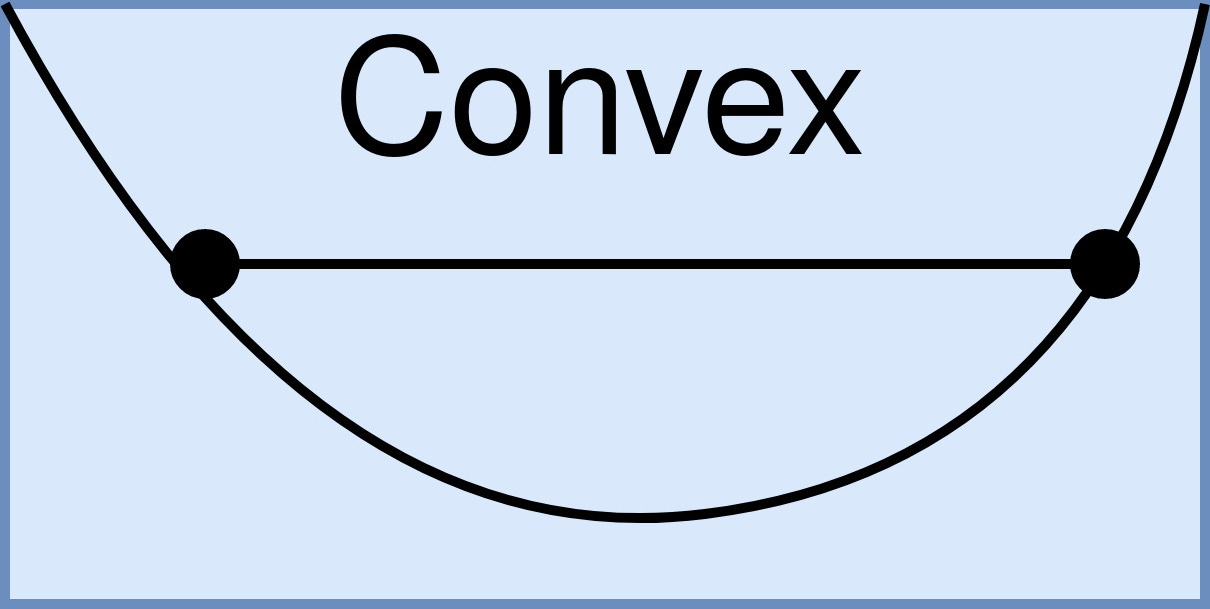
\includegraphics[width=0.5\textwidth]{assets/regression/sr__convex.png}
    \begin{itemize}
      \item \textcolor{black}{One local minimum = global minimum}
      \item \textcolor{black}{Gradient descent works}
    \end{itemize}
  \end{subfigure}\hspace*{0.05\textwidth}
  \begin{subfigure}{0.45\textwidth}
    \centering
    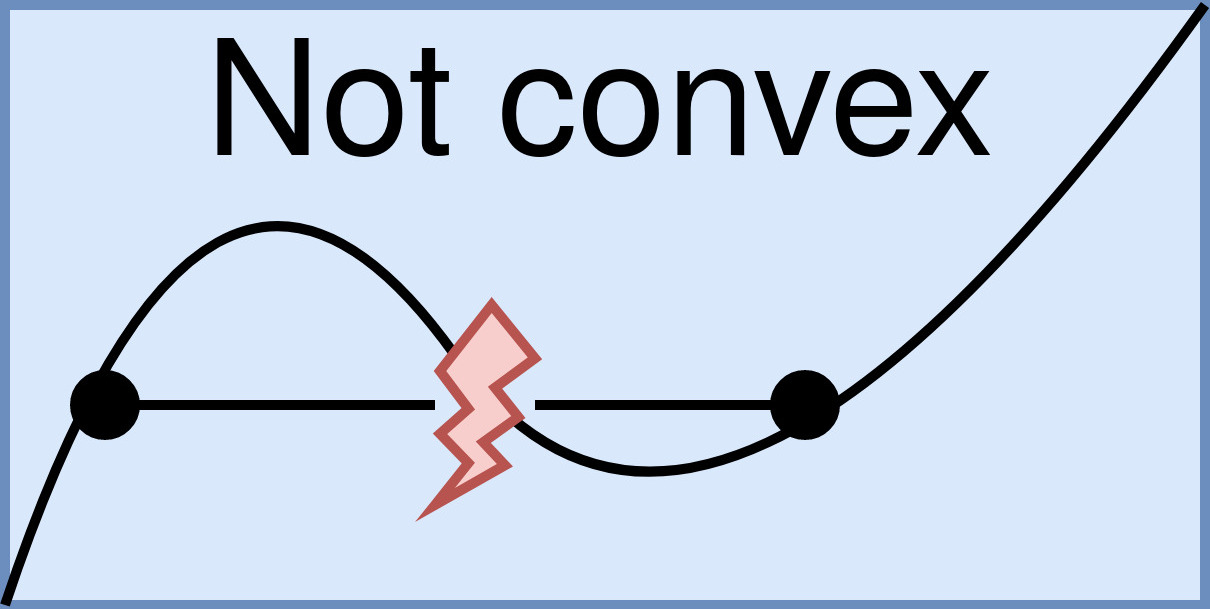
\includegraphics[width=0.5\textwidth]{assets/regression/sr__nonconvex.png}
    \begin{itemize}
      \item \textcolor{black}{Multiple local minima, so global minimum harder to find}
      \item \textcolor{black}{Gradient descent might fail}
    \end{itemize}
  \end{subfigure}
  \caption{Convex vs. non-convex functions}
  \label{fig:4_conv_vs_nonconv}
\end{figure}

The technique we can use to quickly find the global minimum is \textbf{gradient descent}\sidenote{Gradient descent}. For convex functions we know, that we will always end up in the glocal minimum. Still, there is the open question of which direction to walk to:
\begin{itemize}
  \item Take the steepest way down, which is known since there is a derivative of the function.
  \item This leads to a lower point point on each step and therefore converges.
\end{itemize}

An important decision to make is the \textbf{step size}\sidenote{Step size}:
\begin{figure}[H]
  \centering
  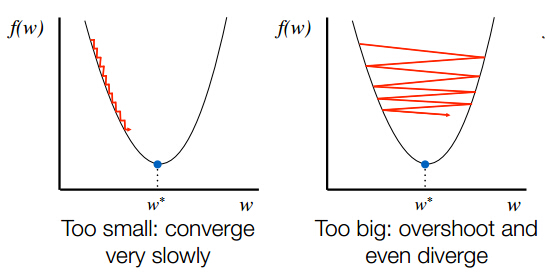
\includegraphics[width=0.6\textwidth]{assets/regression/sr__learning_rate.jpg} 
  \caption{Step size for gradient descent}
  \label{fig:4_learning_rate}
\end{figure}

